\documentclass[11pt,onecolumn,twoside]{report}

\usepackage[
  a4paper,
  twoside,
  top=5mm,                % top margin
  bottom=7mm,             % bottom margin
  inner=20mm,             % inner margin (next to binding)
  outer=20mm,             % outer margin (opposite binding)
  bindingoffset=10mm,     % on binding side
  includeheadfoot,        % include head(er) and foot(er)
  headheight=10mm,        % height of header
  headsep=15mm,           % sep between header and text body
  footskip=15mm,          % sep between body and baseline of footer
  footnotesep = 10mm plus 2mm minus 0mm  % bottom of body to top of footnote
]{geometry}
% A4 paper is w=210m, h=297mm



\newcommand{\fullh}{24cm}         % height of figures for 1 per page
\newcommand{\halfh}{9.5cm}        % height of figures for 2 per page
\newcommand{\thirdh}{6cm}         % height of figures for 3 per page


\setlength{\parindent}{1em}       % less indentation
\setlength{\parskip}{5pt plus 1pt minus 1pt}  % space before a paragraph


% \tolerance is set by LaTeX to 200
% \sloppy sets \tolerance = 9999
% which allows LaTeX more tolerance in adding word spacing

% \sloppy
% \fussy
% \tolerance = 1000

\tolerance=400 
% makes some lines with lots of white space, but      
% tends to prevent words from sticking out in the margin



\setcounter{tocdepth}{3}        % lowest section level entered in ToC
\setcounter{secnumdepth}{3}     % lowest section level still numbered




\usepackage[T1]{fontenc}        % 8-bit output chars (must be before inputenx)
\usepackage[utf8]{inputenx}     % input char encoding

\usepackage[english,austrian,british]{babel}

\usepackage{newtxtext}          % newer times fonts
\usepackage{newtxmath}

\usepackage{relsize}            % relative font sizes \smaller \larger
\usepackage{float}              % H for float placement
\usepackage{setspace}           % line spacing

\usepackage{textcomp}           % symbols such as \texttimes and \texteuro
\usepackage{latexsym}
\usepackage{fontawesome}        % fontawesome symbols

\usepackage{siunitx}            % prettier number formatting
\sisetup{%
  group-separator={,},
}
\usepackage[super]{nth}         % 1st, 2nd, 3rd, etc.

\usepackage{xspace}
\usepackage{xstring}            % string manipulation macros
\usepackage{xparse}             % commands with optional arguments
\usepackage{etoolbox}           % for \newrobustcmd
\usepackage{makecmds}           % for \makecommand
\usepackage{calc}               % for math calculations

\usepackage[svgnames,table,xcdraw]{xcolor}
\definecolor{darkgreen}{rgb}{0.0,0.2,0.0}
\definecolor{darkblue}{rgb}{0.0,0.0,0.2}
\definecolor{darkred}{rgb}{0.2,0.0,0.0}
\definecolor{verylightgrey}{gray}{0.95}
\definecolor{lightgrey}{gray}{0.9}
\definecolor{grey}{gray}{0.7}
\definecolor{black}{gray}{0.0}


\usepackage{longtable}
\usepackage{multirow}
\usepackage{tabularx}

\usepackage{verbdef}            % define robust verb strings
\usepackage{verbatim}
\usepackage{comment}



% better lists
\usepackage{enumitem}

\setlist{
  topsep=0pt,
  partopsep=0pt,
  parsep=0.6ex,
  itemsep=1.2ex,
  left=\parindent .. 2\parindent,    % bullet .. start ot text
}

\setlist[description]{
  style=sameline,
}




\usepackage{listings}                 % for listings of source code

\makeatletter
\newlength{\numwidth}%
\setlength{\numwidth}{\widthof{\normalfont{\lst@numberstyle{99}}}}% Up to 2-digit (99) line numbers
\def\lst@PlaceNumber{%
  \makebox[\numwidth+1em][l]{%
    \makebox[\numwidth][r]{\normalfont\lst@numberstyle{\thelstnumber}}%
  }%
}
\makeatother

% lstset strategy: define defaults here for
% all non-floating listings
% floated listings override these settings later

\lstset{                              % set parameters for listings
  floatplacement=tp,                  % default float placement
  numberbychapter,
  inputencoding=utf8,
  language=,                          % empty = plain text
  basicstyle=\small\ttfamily,
  tabsize=2,
  xleftmargin=2\parindent,
  xrightmargin=2\parindent,
  frame=none,
  framexleftmargin=0mm,
  rulesepcolor=\color{verylightgrey},
  numbers=none,
  numberstyle=\scriptsize,
  numbersep=2ex,
  breaklines,
  showtabs=false,
  showspaces=false,
  showstringspaces=false,
  keywordstyle=\color{black},
  commentstyle=\color{SteelBlue},
  identifierstyle=,
  stringstyle=,
  captionpos=b,
  abovecaptionskip=\abovecaptionskip,
  belowcaptionskip=\belowcaptionskip,
  extendedchars=true,
  literate=%
    {©}{{\textcopyright}}1
    {€}{{\texteuro}}1
    {Ö}{{\"O}}1
    {Ä}{{\"A}}1
    {Ü}{{\"U}}1
    {ß}{{\ss}}1
    {ö}{{\"o}}1
    {ä}{{\"a}}1
    {ü}{{\"u}}1,       % map some utf8 chars for listings
}


\lstdefinelanguage{biblatex}   % based on biblatex v 2.7a from 2013-07-14
{
  keywords={%
    @article,@book,@mvbook,@inbook,@bookinbook,@suppbook,%
    @booklet,@collection,@mvcollection,@incollection,@suppcollection,%
    @manual,@misc,@online,@patent,@periodical,@suppperiodical,%
    @proceedings,@mvproceedings,@inproceedings,@reference,@mvreference,%
    @inreference,@report,@set,@thesis,@unpublished,@xdata,%
    @conference,@electronic,@mastersthesis,@phdthesis,@techreport,@www,%
    @artwork,@audio,@bibnote,@commentary,@image,@jurisdiction,@legislation,%
    @legal,@letter,@movie,@music,@performance,@review,@software,%
    @standard,@video%
  },
  sensitive=false,
  comment=[l][\itshape]{@comment},
  morecomment=[l]{\%},
}

\lstdefinelanguage{CSS}
{
  alsoletter={-},
  morekeywords={%
  color,background,background-color,margin,padding,font,
  font-family,weight,%
  display,position,top,left,right,bottom,list,%
  style,border,size,white,space,min,width%
  },
  sensitive=false,
  morecomment=[l]{//},
  morecomment=[s]{/*}{*/},
  morestring=[b]",
}





\usepackage[compact,nobottomtitles,pagestyles,explicit]{titlesec}
% when using explicit, must explicitly include #1 for titlename

% nobottomtitles
% move section headings close to page bottom to next page
\renewcommand{\bottomtitlespace}{2cm}

% \chaptermark sets the value of \chaptertitle for later
% \@chapapp is defined as \chaptername outside the appendix,
% and as \appendixname within the appendix.
\makeatletter
\titleformat{\chapter}
[display]                                            % shape
{\chaptermark{\thechapter~~#1}\sffamily\bfseries}    % format
{\huge\@chapapp\ \thechapter}                        % label
{4ex}                                                % sep
{\Huge#1}                                            % before-code
\makeatother

\titleformat{name=\chapter,numberless}
[block]                                              % shape
{\chaptermark{#1}\sffamily\bfseries}                 % format
{}                                                   % label
{0ex}                                                % sep
{\Huge#1}                                            % before-code

\titleformat{\section}
{\normalfont\Large\sffamily\bfseries}{\thesection}{0.8em}{#1}

\titleformat{\subsection}
{\normalfont\large\sffamily\bfseries}{\thesubsection}{0.8em}{#1}

\titleformat{\subsubsection}
{\normalfont\normalsize\sffamily\bfseries}{\thesubsubsection}{0.8em}{#1}

\titleformat{\paragraph}[runin]
{\normalfont\normalsize\sffamily\bfseries}{\theparagraph}{0.8em}{#1}

\titleformat{\subparagraph}[runin]
{\normalfont\normalsize\sffamily\bfseries}{\thesubparagraph}{0.8em}{#1}


% vertical spacing before and after section titles
\titlespacing*{\section}
{0pt}{3.5ex plus 0.5ex minus 0.5ex}{0ex plus 0ex minus 0.2ex}

\titlespacing*{\subsection}
{0pt}{2.5ex plus 0.5ex minus 0.5ex}{0ex plus 0ex minus 0.2ex}

\titlespacing*{\subsubsection}
{0pt}{2ex plus 0.5ex minus 0.5ex}{0ex plus 0ex minus 0.2ex}


% define page headings how I want them

\newpagestyle{main}[\small]{
% \addtolength\headheight{6.7pt}
% \headrule
\sethead%
[{\parbox[t]{0.3\textwidth}%                    % even left
  {\sffamily\thepage}}]
[]%                                             % even centre
[{\parbox[t]{0.6\textwidth}%                    % even right
  {\raggedleft\sffamily\chaptertitle}}]
{{\parbox[t]{0.6\textwidth}%                    % odd left
  {\sffamily\sectiontitle}}}%
{}%                                             % odd centre
{{\parbox[t]{0.3\textwidth}%                    % odd right
  {\raggedleft\sffamily\thepage}}}
}



\usepackage{titletoc}

% Add extra per-chapter space to LoL to mimic LoF and LoT
% (requires package etoolbox)
\makeatletter
\patchcmd{\@chapter}% <cmd>
  {\addtocontents}% <search>
  {\addtocontents{lol}{\protect\addvspace{10\p@}}% add per-chapter space
   \addtocontents}% <replace>
  {}{}% <success><failure>
\makeatother

% Configure LoL to mimic LoF and LoT
\contentsuse{lstlisting}{lol}
\titlecontents{lstlisting}
  [3.8em]                      % left indent
  {\addvspace{1.5mm}}          % above-code per entry
  {\contentslabel{2.3em}}      % format for numbered entry
  {\hspace*{-2.3em}}           % format for unnumbered entry
  {\titlerule*[2.7mm]{.} \contentspage}  % dots and page num per entry
  []                           % below-code per entry

\renewcommand{\lstlistlistingname}{List of Listings}





% sensible settings for floats

\setlength{\textfloatsep}{9mm plus 2mm minus 2mm}
\setlength{\floatsep}{9mm plus 2mm minus 2mm}
\setlength{\intextsep}{9mm plus 2mm minus 2mm}

\setlength{\dbltextfloatsep}{9mm plus 2mm minus 2mm}
\setlength{\dblfloatsep}{9mm plus 2mm minus 2mm}

\setlength{\abovecaptionskip}{4mm plus 2mm minus 1mm}
\setlength{\belowcaptionskip}{0mm}

% See http://www-rohan.sdsu.edu/~aty/bibliog/latex/floats.html
% See https://robjhyndman.com/hyndsight/latex-floats/

\setcounter{topnumber}{2}               % max num floats at top of page
\setcounter{dbltopnumber}{2}            % max num floats on 2col page
\setcounter{bottomnumber}{2}            % max num floats at bottom of page
\setcounter{totalnumber}{4}             % max num floats on a page

\renewcommand{\topfraction}{0.8}        % max fraction of floats at top
\renewcommand{\dbltopfraction}{0.9}     % max fraction of floats at top 2col
\renewcommand{\bottomfraction}{0.8}     % max fraction of floats at bottom
\renewcommand{\textfraction}{0.2}       % min fraction of text

% only for entirely float pages:
\renewcommand{\floatpagefraction}{0.7}      % min page fraction having floats
\renewcommand{\dblfloatpagefraction}{0.7}   % min 2col page fraction having floats


% \usepackage[section,above,below]{placeins}  % keep floats to their own section




% use caption and subfig (caption2 and subfigure are now obsolete)

\usepackage[
  position=bottom,
  margin=1cm,
  font=small,
  labelfont={bf,sf},
  format=hang,
  indention=0mm,
]{caption,subfig}

\captionsetup[subfigure]{
  margin=0pt,
  parskip=0pt,
  hangindent=0pt,
  indention=0pt,
  singlelinecheck=true,
  farskip=4mm,            % skip above subfig (assuming captions at bottom)
  captionskip=2mm,        % skip between subfig and subcaption
}


\usepackage[hyphens,obeyspaces]{url}
\def\UrlFont{\smaller\ttfamily}





\usepackage[short]{datetime}   % load datetime *after* babel, requires fmtcount
% \newdateformat{britdate}{%
% \ordinaldate{\THEDAY} \,\monthname[\THEMONTH] \THEYEAR
% }
\newdateformat{unixdate}{%
\twodigit{\THEDAY}~\shortmonthname[\THEMONTH]~\THEYEAR
}



\usepackage[
  autostyle=true,          % adapt quote style to current language
  english=british,         % british english as default
  threshold=1,             % set block quotations >1 line in display mode
  maxlevel=4,              % max nesting level
]{csquotes}

\usepackage[
  indentfirst=false,
  vskip=0pt,               % by default would be \topsep + \partopsep.
]{quoting}

% tell csquotes to use quoting environment
% for \displayquote and \blockquote
\SetBlockEnvironment{quoting}

% if cite is issued by a csquote command
\renewcommand{\mkcitation}[1]{\space#1}

% I prefer double quotes as outer
\DeclareQuoteStyle{keithbritish}%  [variant]{style}
  {\textquotedblleft}%                      opening outer mark
  {\textquotedblright}%                     closing outer mark
  [0.05em]%
  {\textquoteleft}%                         opening inner mark
  {\textquoteright}%                        closing inner mark

\ExecuteQuoteOptions{style=keithbritish}





\usepackage[
  backend=biber,
  style=ext-authoryear,        % defined in biblatex-ext package
  sorting=nyt,
  useprefix,                   % van and von are part of second name
  mergedate=false,             % only for authoryear style
  dashed=false,                % only for authoryear style
  abbreviate=false,
  maxcitenames=2,              % if > 2 authors,
  mincitenames=1,              % use first 1 then et al
  maxbibnames=99,              % if > 99 authors,
  minbibnames=6,               % use first 6 then et al
  uniquelist=minyear,
  uniquename=init,
  hyperref=true,
  backref=true,
  backrefstyle=two,
  sortlocale=en,
]{biblatex}


% set for csquotes, but \autocite only available
% after biblatex is loaded
\SetCiteCommand{\autocite}    % or maybe \parencite

% more space between entries in bib
\setlength\bibitemsep{1.5\itemsep}

% kandrews: replace round brackets with square brackets in citations
\DeclareOuterCiteDelims{parencite}{\bibopenbracket}{\bibclosebracket}
\DeclareInnerCiteDelims{textcite}{\bibopenbracket}{\bibclosebracket}

% kandrews: replace round brackets with square brackets in bibliography
% biblabeldate is a biblatex-ext feature
\DeclareFieldFormat{biblabeldate}{\mkbibbrackets{#1}}


% remove URL: from in front of URLs
\DeclareFieldFormat{url}{\url{#1}}
\DeclareFieldFormat{doi}{\doi{#1}}
\DeclareFieldFormat{isbn}{\isbn{#1}}
\DeclareFieldFormat{issn}{\issn{#1}}

% suppress urldate field
\AtEveryBibitem{\clearfield{urlyear}}

% remove In: from @article and @inproceedings entries
% https://tex.stackexchange.com/questions/10682/suppress-in-biblatex
\renewbibmacro{in:}{%
  \ifboolexpr{%
     test {\ifentrytype{article}}%
     or
     test {\ifentrytype{inproceedings}}%
  }{}{\printtext{\bibstring{in}\intitlepunct}}%
}

% make all entry titles italic
% (also removes quotation marks from around titles)
% https://tex.stackexchange.com/questions/311816/want-title-in-simple-numeric-not-italic-through-bibliography
\DeclareFieldFormat*{title}{\mkbibitalic{#1}}
\DeclareFieldFormat*{citetitle}{\mkbibitalic{#1}}

% make journal names non-italic
\DeclareFieldFormat{journaltitle}{#1\isdot}

% make proceedings names non-italic
\DeclareFieldFormat[inproceedings]{booktitle}{#1\isdot}

% use nth for edition
\DeclareFieldFormat{edition}{%
  \ifinteger{#1}
    {\nth{#1}~\bibstring{edition}}
    {#1\isdot}}

% overwrite some standard strings in english.lbx
\DefineBibliographyStrings{english}{%
  edition          = {Edition},
  mathesis         = {Master's Thesis},
  phdthesis        = {PhD\addabbrvspace Thesis},
}


% kandrews
% use Unix format for dates in biblio:
% 29 Dec 2015, 01 Oct 2018, etc.

% for now, define under lang english not british
% due to bug in biblatex 3.11

\DefineBibliographyStrings{english}{%
  january          = {Jan},
  february         = {Feb},
  march            = {Mar},
  april            = {Apr},
  may              = {May},
  june             = {Jun},
  july             = {Jul},
  august           = {Aug},
  september        = {Sep},
  october          = {Oct},
  november         = {Nov},
  december         = {Dec},
}

\DefineBibliographyExtras{english}{%
% #1 = year, #2 = month, #3 = day
\protected\def\mkbibdatelong#1#2#3{%
  \iffieldundef{#3}
    {}
    {\mkdayzeros{\thefield{#3}}%
     \iffieldundef{#2}{}{\nobreakspace}}%
  \iffieldundef{#2}
    {}
    {\mkbibmonth{\thefield{#2}}%
     \iffieldundef{#1}{}{\space}}%
  \iffieldbibstring{#1}{\bibstring{\thefield{#1}}}{\mkyearzeros{\thefield{#1}}}}%
%
\protected\def\mkbibdateshort#1#2#3{%
  \iffieldundef{#3}
    {}
    {\mkdayzeros{\thefield{#3}}%
     \iffieldundef{#2}{}{\nobreakspace}}%
  \iffieldundef{#2}
    {}
    {\mkbibmonth{\thefield{#2}}%
     \iffieldundef{#1}{}{\space}}%
  \iffieldbibstring{#1}{\bibstring{\thefield{#1}}}{\mkyearzeros{\thefield{#1}}}}%
}


% patch for biblatex 3.11 issue with babel .lbx files
% https://github.com/plk/biblatex/issues/742
% should no longer be necessary with biblatex 3.12
\makeatletter
\protected\long\def\blx@lbx@input@handler@simple#1#2#3#4#5#6{%
  \blx@info@noline{Trying to load #2..}%
  \IfFileExists{#1}
    {\blx@info@noline{... file '#1' found}%
     #3\@@input\@filef@und#4#5%
     \ifcsundef{blx@file@lbx@simple@#1}
       {\listxadd\blx@list@req@stat{#1}%
        \@addtofilelist{#1}%
        \global\cslet{blx@file@lbx@simple@#1}\@empty}
       {}}
    {\blx@info@noline{... file '#1' not found}#6}}

\protected\long\def\blx@lbx@input@handler@once#1#2#3#4#5#6{%
  \ifcsundef{blx@file@lbx@once@#1}
    {\blx@info@noline{Trying to load #2..}%
     \IfFileExists{#1}
       {\blx@info@noline{... file '#1' found}%
        #3\@@input\@filef@und#4#5%
        \ifcsundef{blx@file@lbx@simple@#1}
          {\listxadd\blx@list@req@stat{#1}%
           \@addtofilelist{#1}}
          {}}
       {\blx@info@noline{... file '#1' not found}#6}%
     \global\cslet{blx@file@lbx@once@#1}\@empty
     \global\cslet{blx@file@lbx@simple@#1}\@empty}
    {#5}}
\makeatother




\addbibresource{report.bib}






% adapt pdftitle, pdfsubject, pdfauthor, pdfkeywords
% for your survey paper

\usepackage{ifpdf}

\ifpdf
  % pdflatex
  \usepackage[pdftex]{graphicx}
  \DeclareGraphicsExtensions{.pdf,.jpg,.png}
  \pdfcompresslevel=9
  \pdfpageheight=297mm
  \pdfpagewidth=210mm
  \usepackage[         % hyperref should be last package loaded
    unicode,
    pdftex,
    pdfversion=1.7,
    pdftitle={Writing a Survey Paper},
    pdfsubject={Survey Paper Template},
    pdfauthor={Keith Andrews},
    pdfkeywords={survey paper, skeleton, guidelines, template},
    bookmarks,
    bookmarksnumbered,
    linktocpage,
    colorlinks,
    linkcolor=darkred,
    anchorcolor=red,
    citecolor=darkgreen,
    urlcolor=darkblue,
    pdfview={Fit},
    pdfstartview={Fit},
    pdfpagemode=UseOutlines,       % open bookmarks in Acrobat
    plainpages=false,              % avoids duplicate page number problem
    pdfpagelabels,                 % avoids duplicate page number problem
    breaklinks=true,               % allow links exceeding a single line
  ]{hyperref}

\else
  % latex
  \usepackage[dvips]{graphicx}
  \usepackage[dvips]{hyperref}
  \DeclareGraphicsExtensions{.eps}
\fi



% subset of macros from thesis-macros

% \liintro list item intro is a style used when list items have an
% introduction phrase (say in italics) followed by a colon.
\newcommand{\liintro}[1]{\emph{#1}}

% short notes in square brackets
\newcommand{\shortnote}[1]
{%
{{\smaller{}[#1]}}
}


\newcommand{\TODO}[1]
{
{\textcolor{red}{[TODO: #1]}}
}



\newcommand{\imgcredit}[1]
{\smaller{}[#1]}



\newcommand{\copyrightACM}
{%
Copyright \copyright\ by the Association for Computing Machinery, Inc.%
}




\newcommand{\daymonthyear}[3]
{%
\twodigit{#1}\hspace{0.7ex}\nolinebreak[2]\shortmonthname[#2]\hspace{0.7ex}\nolinebreak[2]#3%
}


\newcommand{\monthyear}[2]
{%
\shortmonthname[#1]\hspace{0.7ex}\nolinebreak[2]#2%
}


\newcommand{\yearmonthday}[3]
{%
\twodigit{#3}\hspace{0.7ex}\nolinebreak[2]\shortmonthname[#2]\hspace{0.7ex}\nolinebreak[2]#1%
}


\newcommand{\yearmonth}[2]
{%
\shortmonthname[#2]\hspace{0.7ex}\nolinebreak[2]#1%
}



% link to Amazon or
% http://worldcatlibraries.org/wcpa/isbn/[ISBN number]
% http://amazon.com/exec/obidos/ASIN/#1/keithandrewshcic
% http://amazon.com/dp/#1/

\newrobustcmd{\isbn}[1]
{%
{%
\ifpdf
{\smaller ISBN
\href{http://amazon.co.uk/dp/#1/}{#1}}%
\else
{\smaller ISBN #1}%
\fi
}%
}



% ISSN
% http://www.bl.uk/services/bibliographic/issn.html
% 8 digits, should be printed xxxx-xxxx
% e.g. 0020-0190 is Information Processing Letters, Elsevier
%
% Lookup services:
% http://kmittlib.lib.kmutt.ac.th:81/search/i?SEARCH=0020-0190
% http://worldcatlibraries.org/wcpa/issn/0020-0190

\newrobustcmd{\issn}[1]
{%
{%
\ifpdf
{\smaller ISSN
\href{http://worldcatlibraries.org/wcpa/issn/#1}{#1}}%
\else
{\smaller ISSN #1}%
\fi
}%
}



% DOIs  http://doi.org/  e.g.
% doi:10.1038/nature723
% http://doi.org/10.1038/nature723

\newrobustcmd{\doi}[1]
{%
{%
\def\UrlFont{\smaller\rmfamily}
\ifpdf                                   % pdflatex
\href{http://doi.org/#1}{doi:\protect\nolinkurl{#1}}%
\else                                    % latex
doi:\protect\nolinkurl{#1}%
\fi
}%
}





\newrobustcmd{\website}[1]
{%
\ifpdf                                  % pdflatex
\href{http://#1/}{\nolinkurl{#1}}%
\else                                   % latex
\nolinkurl{#1}%
\fi
}




\newcommand{\news}[1]
{%
\ifpdf
\href{news:#1}{\nolinkurl{#1}}
\else
\nolinkurl{#1}%
\fi
}








% based on url package
% define styles for class, file, and variable names
% which break nicely at line breaks

% make the macros robust so they work inside captions, etc

\newcommand{\ttname}{\begingroup \smaller\urlstyle{tt}\Url}
\newcommand{\rmname}{\begingroup \smaller\urlstyle{rm}\Url}
\newcommand{\sfname}{\begingroup \smaller\urlstyle{sf}\Url}


% fname is for file names and directory names
\newrobustcmd{\fname}[1]{\ttname{#1}}

% vname is for variable names, domain names, email addresses
\newrobustcmd{\vname}[1]{\ttname{#1}}




% for class names, define our own url style

\makeatletter  % protect @ names

% \url@letstyle: New URL style to premit break at any letters.
% Based on \url@ttstyle

\def\Url@letdo{% style assignments for tt fonts or T1 encoding
\def\UrlBreaks{\do\a\do\b\do\c\do\d\do\e\do\f\do\g\do\h\do\i\do\j\do\k\do\l%
               \do\m\do\n\do\o\do\p\do\q\do\r\do\s\do\t\do\u\do\v\do\w\do\x%
               \do\y\do\z%
               \do\A\do\B\do\C\do\D\do\E\do\F\do\G\do\H\do\I\do\J\do\K\do\L%
               \do\M\do\N\do\O\do\P\do\Q\do\R\do\S\do\T\do\U\do\V\do\W\do\X%
               \do\Y\do\Z%
}%
\def\UrlBigBreaks{\do\.\do\@\do\\\do\/\do\!\do\_\do\|\do\%\do\;\do\>\do\]%
 \do\)\do\,\do\?\do\'\do\+\do\=\do\#\do\:\do@url@hyp}%
\def\UrlNoBreaks{\do\(\do\[\do\{\do\<}% (unnecessary)
\def\UrlSpecials{\do\ {\ }}%
\def\UrlOrds{\do\*\do\-\do\~}% any ordinary characters that aren't usually
\Urlmuskip = 0mu plus 1mu%
}

\def\url@letstyle{%
\@ifundefined{selectfont}{\def\UrlFont{\sf}}{\def\UrlFont{\sffamily}}\Url@letdo
}

\makeatother  % unprotect @ names

% class names
\newcommand\letname{\begingroup \smaller\urlstyle{let}\Url}

\newrobustcmd{\cname}[1]{\letname{#1}}






% Euro symbol
\newcommand{\euro}{\texteuro\,}

% times symbol
\newcommand{\timessym}{\texttimes\,}

% approx symbol
\newcommand{\approxsym}{\ensuremath\approx\,}

% plusminus symbol
\newcommand{\plusminussym}{\textpm\,}

% not equal symbol
\newcommand{\neqsym}{\ensuremath{\neq\,}}

% rightarrow symbol
\newcommand{\rightarrowsym}{\ensuremath\rightarrow\,\,}


% thumbs up and thumbs down symbols

\newcommand{\uthumb}{\smaller[2]\raisebox{1pt}{\textcolor{DarkGreen}{\faThumbsUp}}}

\newcommand{\dthumb}{\smaller[2]\raisebox{1pt}{\textcolor{DarkRed}{\faThumbsDown}}}







\begin{document}

\unixdate

\normalsize
\pagestyle{empty}         % for preliminary pages (no numbers shown)
\pagenumbering{Roman}     % for pdf labels




\begin{titlepage}

\begin{center}
\begin{spacing}{1.1}
\Large\sffamily\bfseries
Diamond:\\
An Online Tool for Card Sorting and Tree Testing
\end{spacing}

\vspace{1cm}

{\large\sffamily Christopher Oser, Markus Ruplitsch, Markus Stradner}

% {\large\sffamily Group 4}
% \vspace{5mm}
% {\large\sffamily Keith Andrews, Tom Strong, Bill Weak, and Seb Green}

\vspace{1cm}

%Institute of Interactive Systems and Data Science (ISDS), \\
%Graz University of Technology \\
%A-8010 Graz, Austria \\[1cm]


 {\large
 706.041 Information Architecture and Web Usability WS 2020/2021 \\
 Graz University of Technology \\[1cm]
 }

\vspace{1cm}

{1 Feb 2021}

\end{center}



\vspace{2cm}

\begin{quote} 
\begin{center} {\large\sffamily\bfseries Abstract} 
\end{center}

This report summarizes the functionalities of Diamond, an application that
offers both, tree testing and card sorting. Since the tree testing capabilities
had already been implemented previously, the focus of this report is an overview
on the new card sorting option that was implemented. Some insights into card
sorting in general as well as the necessary technologies to implement the
application are also provided.

\end{quote}

\vfill

\begin{center}
{\footnotesize\sffamily \copyright ~ Copyright 2021 by the author(s),
except as otherwise noted.}

\vspace{2mm}
{\footnotesize\sffamily This work is placed under a
Creative Commons Attribution 4.0 International
(\href{https://creativecommons.org/licenses/by/4.0/}{CC BY 4.0}) licence.}
\end{center}

\end{titlepage}




\cleardoublepage
\pagestyle{plain}             % for preliminary pages
\pagenumbering{roman}         % for preliminary pages


\begin{spacing}{0.8}
\tableofcontents
\end{spacing}
\addcontentsline{toc}{chapter}{Contents}

\cleardoublepage
\begin{spacing}{0.8}
\listoffigures
\end{spacing}
\addcontentsline{toc}{chapter}{List of Figures}

%\cleardoublepage
%\begin{spacing}{0.8}
%\listoftables
%\end{spacing}
%\addcontentsline{toc}{chapter}{List of Tables}

%\cleardoublepage
%\begin{spacing}{0.8}
%\renewcommand{\lstlistlistingname}{List of Listings}
%\lstlistoflistings
%\end{spacing}
%\addcontentsline{toc}{chapter}{List of Listings}



\cleardoublepage
\pagestyle{main}              % for main pages
\pagenumbering{arabic}        % for main pages

\cleardoublepage
\chapter{Introduction}

\label{chap:Intro}

Diamond: An Online Tool for Card Sorting and Tree Testing was created as an 
extension of the TreeTest tool, which was implemented by Ajdin Mehic as part 
of his Master's Thesis~\parencite{TreeTest}. 
Because of providing both 
functionalities a card sorting tool and a tree testing tool now the application 
was combined under the new name.

In this report you will find a brief introduction to card sorting and an explanation 
of all technologies used to create Diamond. The implementation steps are also 
listed and explained in a constructive manner. Finally, there are expansion 
ideas for the future and final remarks mentioned.


\section{Creating a Card-Sorting Application}

Since there are already many tools out there, it is not easy to find a good 
approach to implement a new app in this sector. One of the best existing 
examples is OptimalSort~\parencite{OptimalSort}.

At Diamond the main target was to keep it simple, but also to equip it with
many features as possible. Therefore, the card sorting process itself is 
designed very intuitive, but also the setup process of a new study is created 
clean and straightforward. Here it is possible to create cards rapidly via 
.csv import.

In addition to editing and deleting, the status of each single study can be 
determined. For this you can switch between launch and unlaunch. For
launched studies you can easily send an invitation link to the users.

Finally, after completition of all the participants, you also have the opportunity 
to export the results as .csv in different ways.



\cleardoublepage
\chapter{Card-Sorting}
\label{chap:Card-Sorting}

In general, card sorting is a technique in user experience. Participants 
of a study have to assign the different cards into the matching 
category, which is more or less a low-tech approach. 

It is mostly used for designing a navigation structure, but it can be used 
for evaluating an information architecture of a website or any other 
information structure, too.
A sample image of card sorting can be viewed in Figure~\ref{fig:sample}. 

\begin{figure}[tp]  \centering
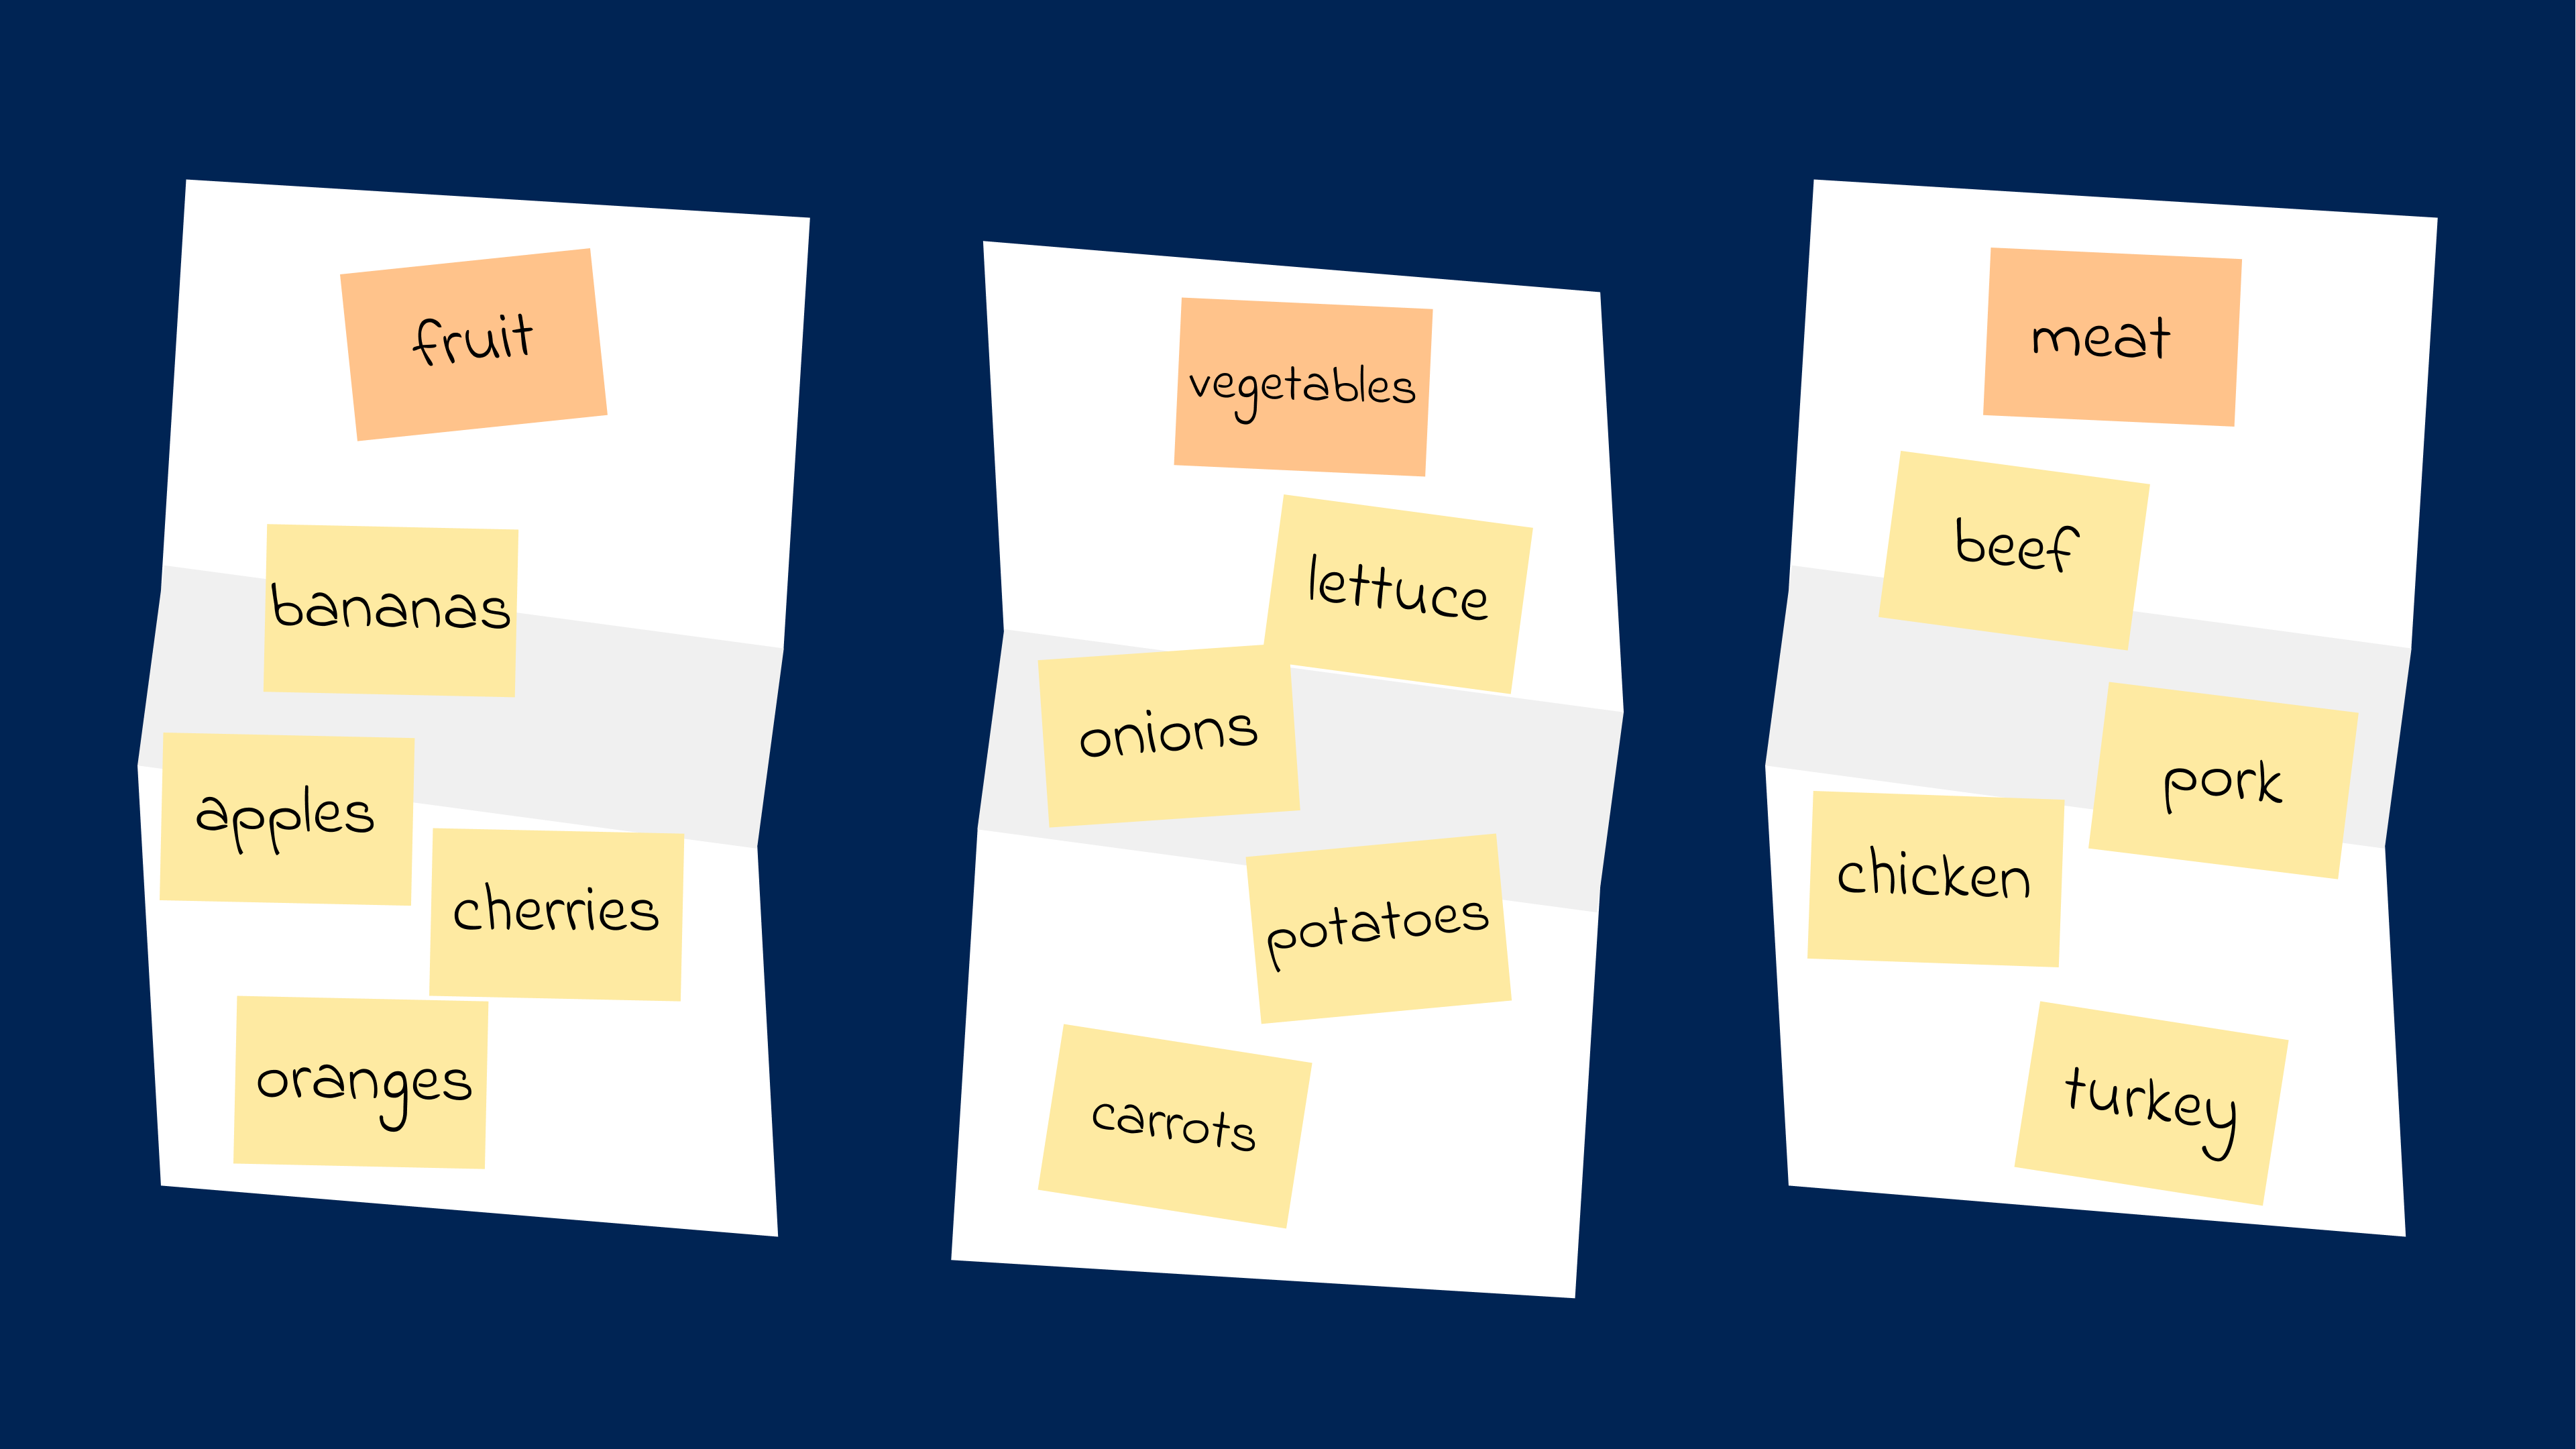
\includegraphics[keepaspectratio,width=\linewidth,height=\halfh]{images/card-sorting/sample.png}
\caption[Sample Image of Card Sorting] 
{A sample image of a card sorting shows dividing cards in three categories.
\imgcredit{Drawn by Markus Stradner, inspired by the illustrations accompanying Sara Jee Watson's blog post  (\url{https://boagworld.com/usability/card-sorting/)}.} } 
\label{fig:sample} 
\end{figure}


\section{Procedure}
All in all, participants of a card sorting study simply assign cards to the 
respective categories, which they believe makes sens. The exact procedure 
depends on the defined variant. 


\section{Variants}
There are three different types of card sorting. At the closed card sorting 
the users have a fixed setup for the categories and at the open card sorting 
they have to create the different categories for their own. But there is also 
a hybrid variant where you actually have a closed card sorting but you are 
also be allowed to add new categories.  








\cleardoublepage
\chapter{Technologies}
\label{chap:Tech}

This chapter covers the different frameworks and technologies that were used to
create Diamond. While many of these technologies provide a wide array of
features, only the features used during the development of Diamond will be
mentioned here. For more in-depth information it is suggested to have a look
at the different documentations.

\section{Angular}

Angular is one of the most popular design frameworks for web applications.
Angular applications are structured in such a way that each visible part of the
app has its own .css, .html and .ts file and is called a component. As with 
other web applications the typescript file contains the logic, the HTML file 
contains the markup and the CSS file defines the look and feel of the component.
TreeTest was originally written in Angular 7 and was updated to the newest 
version of Angular (Angular 11) before development of Diamond began.

\section{Node.js}

Node.js is a JavaScript runtime environment that was used to set up the server 
side of application. It simplifies many of the different web protocol 
interactions and allows developers to handle requests and responses 
asynchronously without having to implement multi threading themselves. Node.js 
was also used to store and retrieve the information stored on the MongoDB 
database.

Additionally, npm is a package manager that comes with Node.js by default, and 
was used to clone all used packages and keep them up-to-date during 
development. This makes the use of external libraries significantly easier and 
reduces the overhead when committing changes to git.

\section{MongoDB}

To store all user related information a MongoDB database was set up. The 
communication between our server and the database was handled by Node.js. 
Furthermore, MongoDB compass was used to visualize the database and manually 
interact with it, in case some erroneous information was stored. A screenshot 
can be seen in Figure~\ref{fig:mongodb_compass}. 


\begin{figure}[tp]  \centering
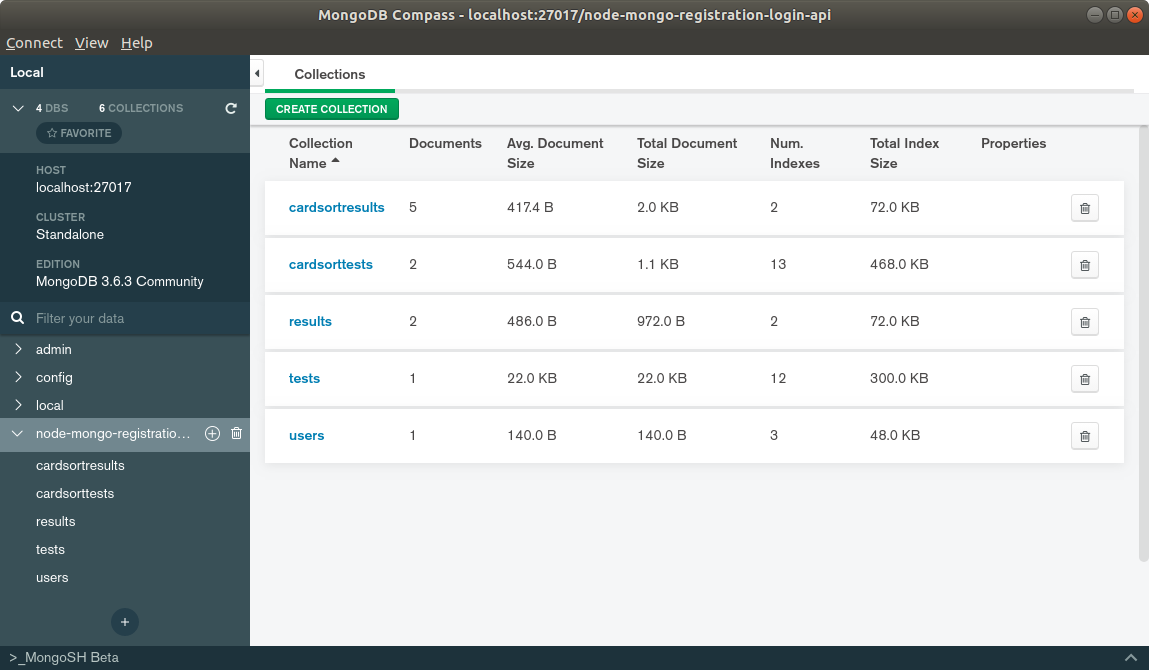
\includegraphics[keepaspectratio,width=\linewidth,height=\halfh]{images/technologies/mongodb_compass.png}
\caption[MongoDB Compass] 
{MongoDB Compass showing the database with some stored information
\imgcredit{Screenshot was captured by Markus Ruplitsch using
MongoDB Compass.} } 
\label{fig:mongodb_compass} 
\end{figure}

\section{Heroku}

Heroku was used for online hosting. In general it is a container-based 
cloud Platform as a Service (PaaS). This means that everything about 
setting up a server, online deployment and hosting is provided by it. It 
is very intuitive to use and free of charge, but an account is needed. 

Heroku offers to connect a GitHub repository to that account. This is 
quite convenient, because you can choose a branch to enable 
auto-deployment after every single push on this branch. For this reason 
you can keep your web application up-to-date very easily. 

It is recommended to created an Heroku branch and to push on that 
branch, when there is a larger number of changes to deploy online. 
And the main branch should just be configured with the localhost 
settings for testing locally.



\cleardoublepage
\chapter{Implementation}

\label{chap:Implem}


In this chapter the core functionalities of the card sorting capabilities of
Diamond are presented. Most importantly, the actual sorting implementation is 
explained. Furthermore, all other aspects, such as creating a card sort study
or exporting and possible analytics of the results are also discussed.


\section{Creating a Card Sort}

The main structure of card sort study creation was taken from the previously 
implemented TreeTest, but it was not copied entirely. Adjustments were made to
better represent a card sort study. 

Every study has a name and an option to include a mandatory password to guard
the study from unwanted participants. Then a welcome message, instructions as
well as a thank you message and feedback message can be specified. These
messages are customizable to facilitate easy adjustments according to the needs
of the respective study.

Cards can be added manually through an input text field. After creation there is
also the possibility of renaming or deleting previously added cards. Another way
of loading the wanted cards is by importing the dataset via a .csv file. Here 
any number of cards, separated by a comma or semicolon, are included into the
study card list for later sorting. Note that using the import function clears
any previously added cards, as this helps unintentionally mixing datasets.

A screenshot of the card sort creation can be viewed in
Figure~\ref{fig:creation}. 


\begin{figure}[tp]  \centering
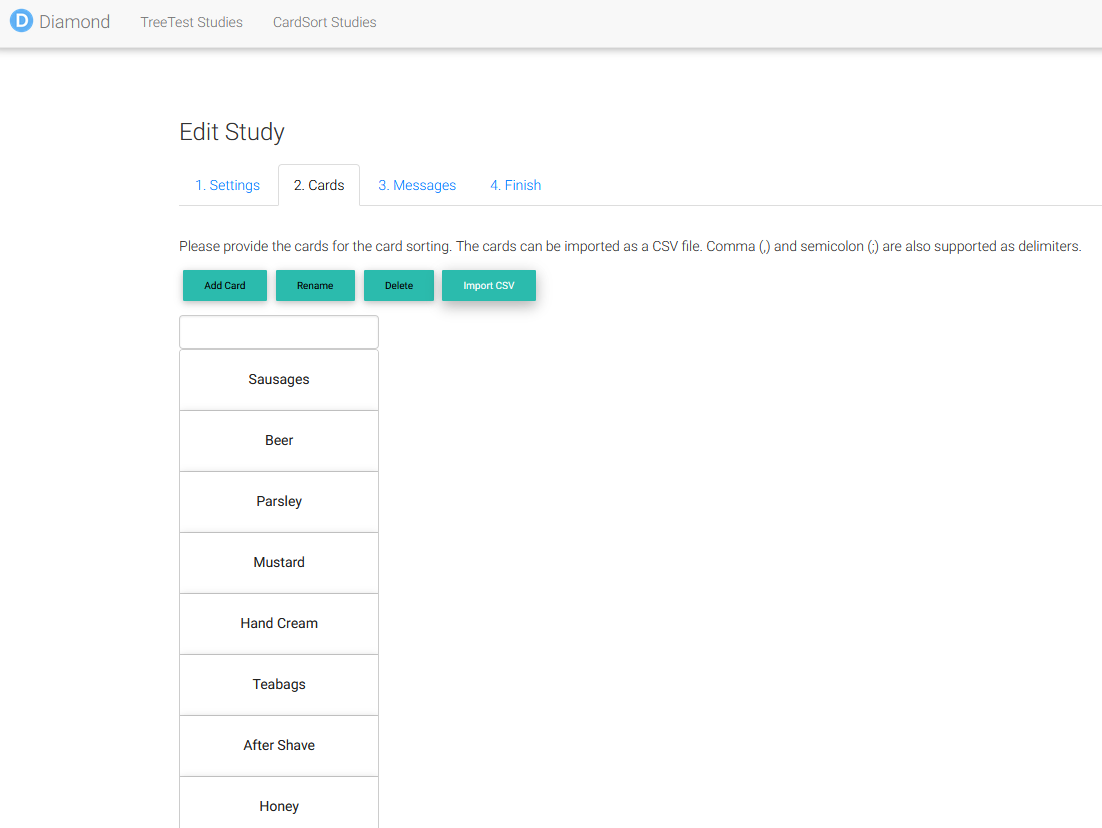
\includegraphics[keepaspectratio,width=\linewidth,height=\halfh]{images/implementation/create.png}
\caption[Card Sort Study Creation] 
{The graphical user interface during the adding of cards to a card sort study.
\imgcredit{Screenshot was captured by Christopher Oser using
Diamond.} } 
\label{fig:creation} 
\end{figure}

\section{Taking part in a Study}

Once a card sort study has been created, it is possible to share it to users.
This can be done via a link and possibly a password to further control the users
taking part in the study. Each user needs to specify their name and receives
the previously defined welcome message and instructions before attempting the
actual sorting.

The card sorting itself is made up of the card list, which is presented to the
user on the left of the screen, and a dedicated area for groups that are to be
defined by the user. The cards in the card list are stacked vertically and the
remaining amount of cards in the list can be seen at the very top.  

Currently Diamond only supports open card sorting, which, according to Prof.
Keith Andrews, ``..is the only true form of card sorting''. Therefore all groups
need to be defined by the user. This can be done via a input text field. Once a
group is added, cards can be dragged from the card list to a group of choice.
All groups can be renamed or deleted. Did a deleted group contain cards, these
cards are then added back to the card list to be sorted again. A screenshot of
the card sorting process can be viewed in Figure~\ref{fig:sorting}.

\begin{figure}[tp]  \centering
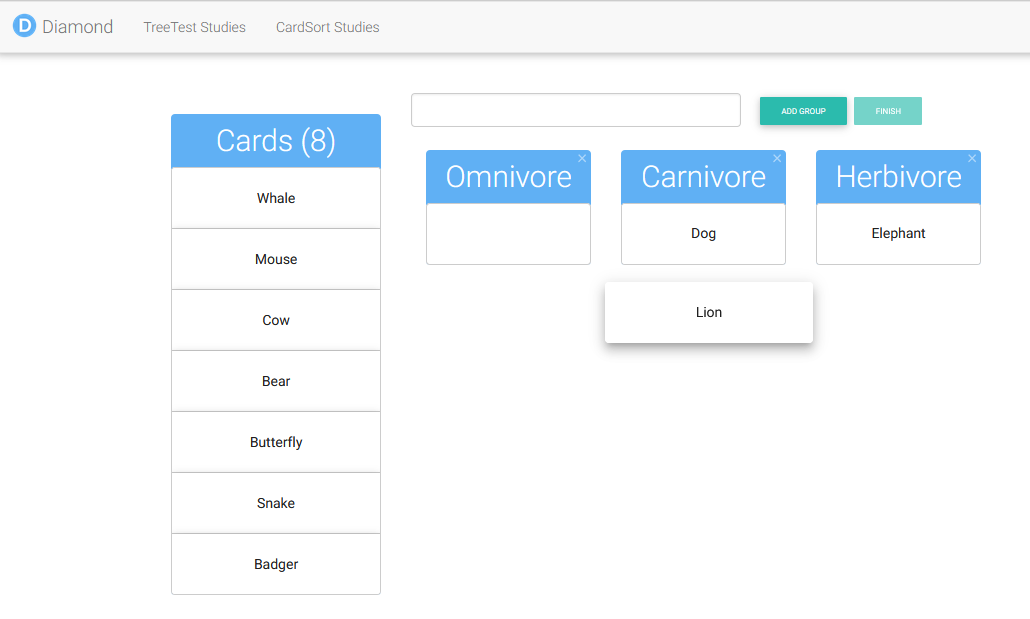
\includegraphics[keepaspectratio,width=\linewidth,height=\halfh]{images/implementation/sorting.png}
\caption[Card Sorting Interface] 
{The graphical user interface during the sorting of cards by the user.
\imgcredit{Screenshot was captured by Christopher Oser using
Diamond.} } 
\label{fig:sorting} 
\end{figure}

Once all cards have been assigned to groups the user has the option to finish
their sort. The next step for the user is to explain their mindset during the
sorting, to facilitate better analytics of the results. After this, the user is
presented with the option to provide general feedback concerning the study.

\section{Evaluating Results}

At any point during the study, the study manager, the person who created the
study, can view and export the results of the study. The results are composed by
the name of the user, the date of the sorting, the sorting results, the mindset
and the feedback message. The general overview of the results of a study can be
viewed in Figure~\ref{fig:results}. The sorting results are displayed on a
separate page for each user, they are made up by a table where each column
represents one group. A sample table can be viewed in Figure~\ref{fig:table}.

The results can also be exported for later use in .csv format. There are two
different files that are ready for export. The first is the user data, comprised
by names, dates, feedback messages and mindsets. The data is represented per row
per user. The second file is the sorting data over all users. Here the data is
represented by all cards in the first row, followed by a one user per row group
assignment to the respective card in the column. So each user's sorting data is
represented by a row of groups.

\begin{figure}[tp]  \centering
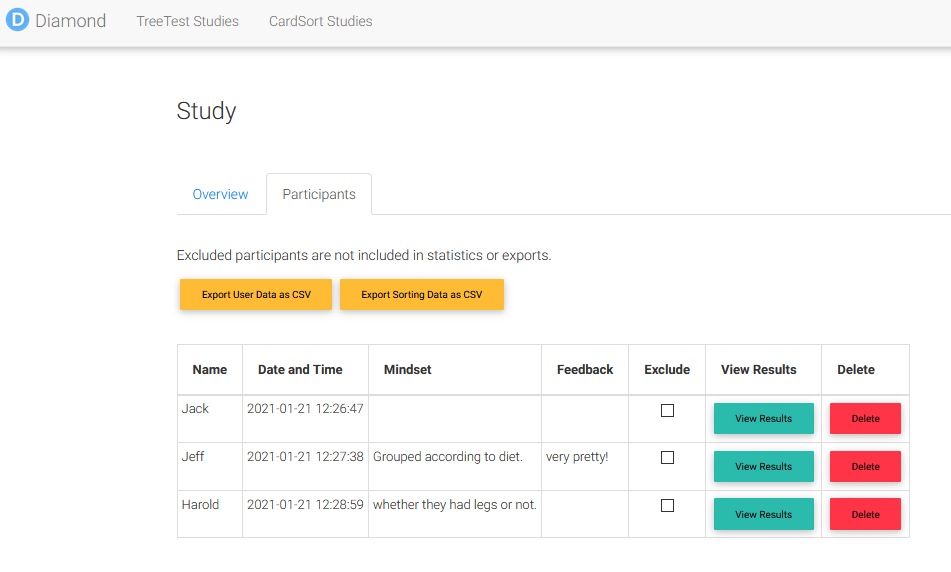
\includegraphics[keepaspectratio,width=\linewidth,height=\halfh]{images/implementation/results.png}
\caption[Card Sorting Results Overview] 
{The overview over the results of a card sort study in Diamond.
\imgcredit{Screenshot was captured by Christopher Oser using
Diamond.} } 
\label{fig:results} 
\end{figure}

\begin{figure}[tp]  \centering
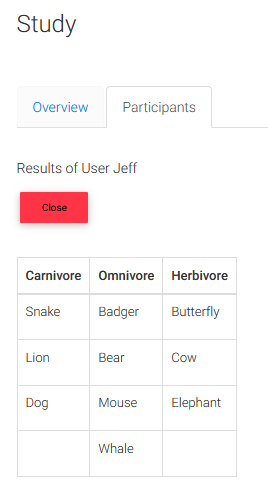
\includegraphics[keepaspectratio,width=\linewidth,height=\halfh]{images/implementation/table.png}
\caption[Card Sorting Result Table] 
{The table that represents the sorting results of one user. Each group is represented
by a column and the respective cards are listed below the first row.
\imgcredit{Screenshot was captured by Christopher Oser using
Diamond.} } 
\label{fig:table} 
\end{figure}

\cleardoublepage
\chapter{Conclusion}

\label{chap:Concl}

Now that all the details of the implementation of Diamond have been covered, 
this chapter concludes the report and ends with some possible improvement for 
the future and some final remarks.

\section{Possible Improvements}

Due to limited time, some features, which are present in many other card 
sorting applications, were not implemented. Here is a short list of features we 
thought of:

\begin{itemize}
  \item Currently, the only information on the participants that is stored is 
  their name. It could be interesting to give the creator of a study the 
  possibility to create custom questionnaires  to extract more information 
  about the participants
  \item It would be nice to allow users to decide whether they want to create 
  an open, close or hybrid card sorting study. This could be done with only 
  minor additional effort. 
  \item While an overview of the results is provided within the app, for most 
  use cases it is necessary to export the results and then import them into some
  third application for further evaluation. The tracking and display of 
  statistics such as average sorting duration or how often users changed their 
  minds when sorting cards would be quite helpful and interesting.
  \item It might be interesting to create sub-groups when sorting the cards. 
  This would require rescaling the size of the groups during the sorting process
  and abstracting the cards into another component.
\end{itemize}



\section{Final Remarks}

As of the time of writing this report, Diamond is hosted publicly on Heroku 
under \url{https://iaweb-diamond.herokuapp.com/#/tests}.

The git repository is 
\url{https://github.com/somestudentcoder/Diamond}.





\cleardoublepage
% for now, switch to language english
% hack to force unix date for biblio, biblatex 3.11
\begin{otherlanguage}{english}
\printbibliography[heading=bibintoc]
\end{otherlanguage}


\end{document}

